\documentclass[11pt]{article}
\usepackage[margin=1in]{geometry}
\usepackage[T1]{fontenc}
\usepackage[utf8]{inputenc}
\usepackage{lmodern}
\usepackage{amsmath}
\usepackage{graphicx}
\usepackage{booktabs}
\usepackage[hidelinks]{hyperref}
\usepackage{microtype}
\usepackage[font=small,labelfont=bf]{caption}

% generated from results/ by paper/make_numbers.py -- do not edit
\newcommand{\NNeuronsTotal}{139{,}255}
\newcommand{\NPairs}{3{,}732{,}460}
\newcommand{\Neurons}{133}
\newcommand{\Edges}{650}
\newcommand{\Inputs}{52}
\newcommand{\Outputs}{63}
\newcommand{\Intermediates}{18}
\newcommand{\ExcPct}{62.8}
\newcommand{\Reciprocity}{0.34}
\newcommand{\NAch}{400}
\newcommand{\NGaba}{46}
\newcommand{\NGlut}{196}
\newcommand{\NMono}{8}
\newcommand{\NParams}{157}
\newcommand{\NSeeds}{10}
\newcommand{\TestGames}{500}
\newcommand{\BudgetSteps}{4{,}000{,}000}
\newcommand{\TrainTime}{70}
\newcommand{\ConnMean}{27.3}
\newcommand{\ConnSd}{3.6}
\newcommand{\ConnMin}{22.2}
\newcommand{\ConnMax}{33.1}
\newcommand{\ConnMaxLen}{53}
\newcommand{\ConnStepsPerFood}{18.7}
\newcommand{\DegMean}{26.9}
\newcommand{\DegSd}{2.4}
\newcommand{\DegP}{0.91}
\newcommand{\ErMean}{26.0}
\newcommand{\ErSd}{2.0}
\newcommand{\ErP}{0.47}
\newcommand{\SignMean}{25.7}
\newcommand{\SignSd}{3.7}
\newcommand{\SignP}{0.62}
\newcommand{\NoRecMean}{28.9}
\newcommand{\NoRecSd}{2.9}
\newcommand{\NoRecP}{0.31}
\newcommand{\NoRaysMean}{25.9}
\newcommand{\NoRaysSd}{2.6}
\newcommand{\ASeventyMean}{27.5}
\newcommand{\ATwoEightyMean}{26.5}
\newcommand{\NeuronsSeventy}{73}
\newcommand{\NeuronsTwoEighty}{278}
\newcommand{\GreedyMean}{18.4}
\newcommand{\FloodMean}{68.8}
\newcommand{\RandMean}{0.2}
\newcommand{\DeathBody}{56.5}
\newcommand{\DeathTrapped}{43.4}
\newcommand{\DeathWall}{0.0}
\newcommand{\DeathTimeout}{0.1}
\newcommand{\LesTopBelow}{3}
\newcommand{\LesSeeds}{10}
\newcommand{\LesK}{7}
\newcommand{\VOneMean}{17.1}
\newcommand{\VOneSd}{9.0}
\newcommand{\VOneNeurons}{278}


\title{\textbf{A Fly Visual-to-Motor Circuit Plays Snake:\\a Minimal Connectome-Constrained Controller}}
\author{Burak G\"ulmez\\[2pt]
\small College of Engineering and Architecture, University College Dublin, Dublin, Ireland\\
\small \texttt{burak.gulmez@ucd.ie}}
\date{}

\begin{document}
\maketitle

\begin{abstract}
\noindent
The FlyWire reconstruction of an adult \textit{Drosophila} brain makes it possible to use measured
wiring, rather than an arbitrary architecture, as the recurrent core of an artificial agent. In this
study, \Neurons{} neurons lying on short paths from visual projection neurons to descending neurons
are extracted, their \Edges{} connections are converted into fixed weights from synapse counts and
predicted neurotransmitters, and a trainable interface of \NParams{} parameters is attached. Only
that interface is optimised, by an evolution strategy, in roughly one minute per run on a laptop
CPU, while the connectome weights stay frozen. The resulting agent plays Snake on a $10\times10$
grid: \ConnMean{}~$\pm$~\ConnSd{} food items are eaten per game over \TestGames{} unseen games and
\NSeeds{} independent runs, and no game ends at a wall. Degree-preserving shuffles,
Erd\H{o}s--R\'enyi graphs, sign-shuffled weights and a network without recurrent connections reach
the same score range, so no measurable benefit of the measured wiring is found on this task. The
agent, the controls and the main failure mode (self-collisions) are reported as a small, fully
reproducible case study rather than as evidence about fly computation.
\end{abstract}

\textbf{Keywords:} connectome; \textit{Drosophila}; FlyWire; recurrent network; evolution strategy; game agent

\section{Introduction}
Electron-microscopy reconstructions now provide synapse-level wiring diagrams of entire insect
brains. The FlyWire dataset describes $5\times10^{7}$ chemical synapses between 139{,}255 neurons of
an adult female \textit{Drosophila melanogaster} \cite{dorkenwald2024}. It is accompanied by
whole-brain annotations of cell classes and types \cite{schlegel2024} and by neurotransmitter
identities predicted from the electron-microscopy images \cite{eckstein2024}. Such data invite a
simple question: if the wiring is fixed and only the coupling to the outside world is learned, what
behaviour can a measured circuit support?

Related work has mostly been aimed at explaining neural activity or function. A model of the fly
motion pathways built on measured connectivity, with unknown single-neuron and synapse parameters
optimised for motion detection, was shown to predict recorded neural responses
\cite{lappalainen2024}. Control-theoretic analysis of the \textit{C.\ elegans} connectome was used to
predict which neurons are involved in locomotor behaviour \cite{yan2017}. In the present study a
different angle is taken: a connectome fragment is placed in a closed loop with a game. Snake is
convenient because the rules are short, the state is small, and strong reference strategies are easy
to write by hand. Games of this kind are usually approached with deep reinforcement learning, as in
the Atari benchmark \cite{mnih2015} and in Snake itself \cite{wei2018}. Maximum performance is not
the aim here; the learned part is kept as small as possible so that whatever the agent does rests
mainly on the fixed circuit.

The setup is close in spirit to reservoir computing, in which a fixed random recurrent network is
combined with a trained readout \cite{jaeger2004}. The difference is that the reservoir used here is
not random: it is a measured piece of the fly brain. It starts at visual projection neurons, which
convey information on the presence and location of visual features to the central brain and whose
activation can evoke avoidance-like and turning behaviours \cite{wu2016}, and it ends at descending
neurons. Matched random and shuffled reservoirs are therefore also trained as controls.

Three contributions are made: (i) a laptop-scale, fully seeded pipeline from FlyWire tables to a
closed-loop Snake agent; (ii) a comparison of the measured circuit with four matched alternatives
under an identical training budget; and (iii) a negative result on the role of the wiring, released
with code, logged results and a browser demo that reproduces the reported games exactly.

\section{Methods}

\paragraph{Circuit.}
Connection rows of the FlyWire v783 Codex export were summed per neuron pair, which gave \NPairs{}
connected pairs among \NNeuronsTotal{} neurons. Visual projection neurons were treated as sources
and descending neurons as targets. Only pairs with at least 200 synapses were considered, and every
neuron on a path of at most two steps from a source to a target was retained: \Inputs{} inputs,
\Outputs{} outputs and \Intermediates{} intermediate neurons (\Neurons{} in total). All \Edges{}
connections with at least five synapses between the retained neurons were kept, with weight
$W_{ij}=\pm\log(1+n_{ij})$ for $n_{ij}$ synapses. Signs were assigned from the predicted transmitter
of the presynaptic cell \cite{eckstein2024}: acetylcholine positive (\NAch{} connections), GABA
(\NGaba{}) and glutamate (\NGlut{}) negative, monoamines (\NMono{}) positive. The matrix was rescaled
to spectral radius $0.9$; \ExcPct\% of its connections are excitatory (Fig.~\ref{fig:circuit}).

\paragraph{Task.}
The board is $10\times10$ and the snake starts with length three. At each step a left turn, a right
turn or a straight move is chosen. Food is placed on a uniformly random free cell drawn from a seeded
32-bit xorshift generator, so that a seed fixes the whole game. A game ends on a wall or body
collision, or after 200 steps without food. A death is additionally labelled \emph{trapped} if no
safe action existed at that moment.

\paragraph{Sensors and network.}
Fifteen readings are computed in the head frame: the signed forward and lateral offset of the food,
its normalised distance and four quadrant flags; three flags for an immediate collision; the inverse
distance to the first obstacle along each of the three directions; and two diagonal occupancy flags.
Neuron states follow $x \leftarrow x + a\,(-x + g\,W\tanh(x) + I)$ with ten updates per game step,
where $I$ is constant within each of eight input groups. Three action scores are read from the mean
activity of eight output groups, and the largest is selected. The trainable parameters are the input
map, the readout, the leak $a$ and the gain $g$: \NParams{} values. Training was performed with
CMA-ES \cite{hansen2001} (population 16, four games per candidate) and stopped after \BudgetSteps{}
game steps, about \TrainTime{}\,s per run on eight CPU cores. Disjoint seed ranges were used for
training, validation and test games, and every configuration was repeated with \NSeeds{} seeds.

\paragraph{Controls.}
With identical sensors, interface and budget, $W$ was replaced by a degree-preserving shuffle, by an
Erd\H{o}s--R\'enyi graph of the same size, by the same graph with excitatory and inhibitory signs
permuted, and by $W=0$, in which case the action is read directly from the driven input groups.

\begin{figure}[t]
\centering
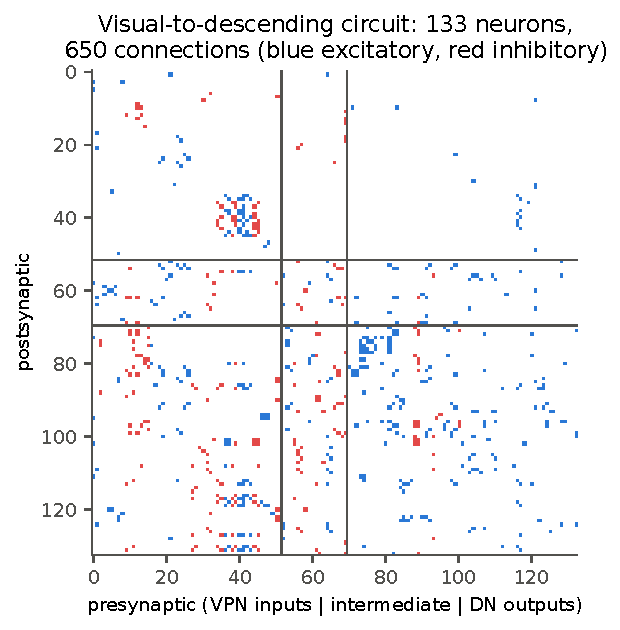
\includegraphics[width=0.42\linewidth]{../figures/fig1_circuit.pdf}\hfill
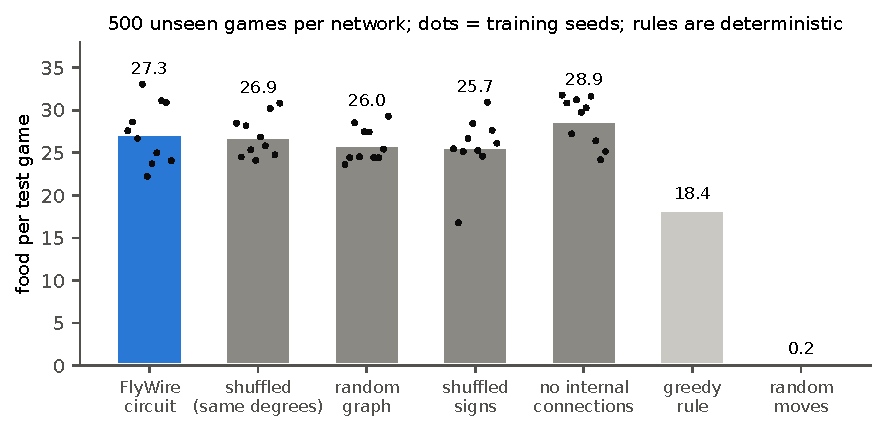
\includegraphics[width=0.55\linewidth]{../figures/fig3_comparison.pdf}
\caption{Left: the extracted circuit (inputs, intermediates, outputs; blue excitatory, red
inhibitory). Right: food per test game; dots are independent training runs, the two right-hand bars
are deterministic reference rules.}
\label{fig:circuit}
\end{figure}

\section{Results}
On average \ConnMean{}~$\pm$~\ConnSd{} food items per test game were eaten by the trained networks
(range \ConnMin{}--\ConnMax{} across runs; longest snake \ConnMaxLen{} cells; \ConnStepsPerFood{}
steps per food). A greedy hand-written rule that moves toward the food unless the move is immediately
fatal reached \GreedyMean{}, and uniformly random actions reached \RandMean{}. A flood-fill rule that
also keeps the tail reachable, included only as a strong reference, reached \FloodMean{}.

Games almost never ended at a wall (\DeathWall\%) or in a timeout (\DeathTimeout\%). Instead,
\DeathBody\% ended with the snake entering its own body although a safe action was available, and
\DeathTrapped\% ended with no safe action left. The static boundary is thus learned quickly, whereas
the growing body is handled poorly (Fig.~\ref{fig:game}).

Little changed when the measured wiring was replaced: \DegMean{}~$\pm$~\DegSd{} was obtained for the
degree-preserving shuffle, \ErMean{}~$\pm$~\ErSd{} for the random graph, \SignMean{}~$\pm$~\SignSd{}
for shuffled signs and \NoRecMean{}~$\pm$~\NoRecSd{} without recurrence. None of these differed
clearly from the connectome (two-sided Mann--Whitney tests over runs: $p=\DegP$, $\ErP$, $\SignP$,
$\NoRecP$). Circuits of \NeuronsSeventy{} and \NeuronsTwoEighty{} neurons obtained with the same rule
scored \ASeventyMean{} and \ATwoEightyMean{}, and \NoRaysMean{}~$\pm$~\NoRaysSd{} was obtained when
the three obstacle-distance readings were removed. Silencing the \LesK{} most active neurons was
worse than silencing the same number at random in only \LesTopBelow{} of \LesSeeds{} runs.

\begin{figure}[t]
\centering
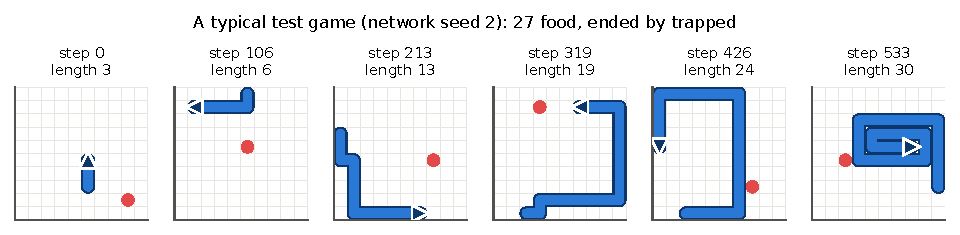
\includegraphics[width=\linewidth]{../figures/fig4_example_game.pdf}
\caption{Snapshots of one test game; the triangle marks the head and its heading.}
\label{fig:game}
\end{figure}

\section{Discussion}
Snake is played at beginner level by a frozen fragment of fly wiring with \NParams{} trained numbers.
The comparison with matched graphs shows that, in this setting, the specific connectivity is not what
makes it work: most of the task is already carried by the hand-designed sensors and the small
trained map, which is why the recurrence-free variant performs equally well. This is a statement
about the setup, not about the fly. The task is unrelated to the natural function of these neurons,
spiking dynamics are collapsed into a rate variable, transmitter-based signs are predictions rather
than measurements \cite{eckstein2024}, and the circuit selection rule (two synapses, strong
connections) is one choice among many. The picture might change with a richer task, a longer budget,
or a readout constrained to biologically meaningful cell types. The dominant failure mode, running
into the snake's own body, suggests that memory of the recent trajectory is the missing ingredient.

\section{Conclusion}
Connectome-derived wiring can be placed into a closed-loop game agent at laptop scale, and the agent
works, but on Snake it is not better than a random graph of the same size.

\paragraph{Data and code availability.} FlyWire v783 tables are distributed through the FlyWire
Codex \cite{dorkenwald2024, schlegel2024}. The code, configuration files, per-run logs and the
browser demo are available at \url{https://github.com/burakgulmez/fly-snake}.

\bibliographystyle{plain}
\bibliography{refs}
\end{document}
